%% --------------------------------------------------------------------------
% LaTeX template for the XLI CILAMCE.
%
% This latex document tries to copy the Microsoft Word template.
% --------------------------------------------------------------------------
\documentclass[a4paper,10pt]{book}

% PACKAGES USED - packages that need to be previously installed on your computer
\usepackage[lmargin=2.5cm, rmargin=2.5cm, tmargin=2.5cm, bmargin=2.5cm ]{geometry}
\usepackage{graphicx}
\usepackage{times}
\usepackage{indentfirst}
\usepackage{fancyhdr}
\usepackage{titlesec}
\usepackage[english]{babel}
\usepackage{parskip} 
\usepackage{setspace}



%%%%%%%%%%%%%%%%%%%%%%%%%%%%%%%%%%%%%%%%%%%%%%%%%%%%%%%%%%%%%%%%%
%%%%%%%%%%%%%%%%%%%%%%%%%%%%%%%%%%%%%%%%%%%%%%%%%%%%%%%%%%%%%%%%%
%%% My Additional Packages
%%%%%%%%%%%%%%%%%%%%%%%%%%%%%%%%%%%%%%%%%%%%%%%%%%%%%%%%%%%%%%%%%
\usepackage[utf8]{inputenc}
%\usepackage{amssymb} %Mathematics
%\usepackage{amsfonts}%Mathematics
%\usepackage{amsmath,amscd}%Mathematics
%\usepackage{amsthm}%Mathematics
%\usepackage{mathrsfs}%Mathematics font
%\usepackage{xspace}
%\usepackage{booktabs}
%\usepackage{stmaryrd}%Particular Brackets
%\usepackage{graphicx} %Tables and Figures
%\usepackage{subfigure}
%\usepackage{url}
\usepackage{hyperref}
\usepackage{cleveref}
\usepackage{./pkg-crefNames}
\usepackage[labelsep=period]{caption}

%BibTeX compatible with the CILAMCE format
\usepackage[numbers,sort&compress]{natbib}

\setlength{\bibsep}{0pt plus 0.3ex}

\renewcommand*{\bibfont}{\small}

\makeatletter
\renewcommand\bibsection
{
  \section*{References}
}



\renewenvironment{thebibliography}[1]
      {\section*{\refname}%
       \@mkboth{\MakeUppercase\refname}{\MakeUppercase\refname}%
       \list{\@biblabel{\@arabic\c@enumiv}}%
            {\settowidth\labelwidth{\@biblabel{#1}}%
             \leftmargin\labelwidth
             \advance\leftmargin-10pt% change 20 pt according to your needs
             \advance\leftmargin\labelsep
             \setlength\itemindent{10pt}% change using the inverse of the length used before
             \@openbib@code
             \usecounter{enumiv}%
             \let\p@enumiv\@empty
             \renewcommand\theenumiv{\@arabic\c@enumiv}}%
       \sloppy
       \clubpenalty4000
       \@clubpenalty \clubpenalty
       \widowpenalty4000%
       \sfcode`\.\@m}
      {\def\@noitemerr
        {\@latex@warning{Empty `thebibliography' environment}}%
       \endlist}
\renewcommand\newblock{\hskip .11em\@plus.33em\@minus.07em}
\makeatother




\makeatother
\bibliographystyle{bib-cilamce}
%\bibliographystyle{plain}


%%%%%%%%%%%%%%%%%%%%%%%%%%%%%%%%%%%%%%%%%%%%%%%%%%%%%%%%%%%%%%%%%
%%%%%%%%%%%%%%%%%%%%%%%%%%%%%%%%%%%%%%%%%%%%%%%%%%%%%%%%%%%%%%%%%

% CONFIGURATION
\renewcommand*\arraystretch{1.5}
\renewcommand*\thesection{\arabic{section}}
%\hyphenpenalty=10000 % You can uncomment this to avoid hyphenization
\titleformat*{\section}{\large\bfseries}
\titleformat*{\subsection}{\bfseries}
\titlespacing\section{0pt}{20pt plus 2pt minus 2pt}{12pt plus 2pt minus 2pt}
\titlespacing\subsection{0pt}{20pt plus 0pt minus 0pt}{12pt plus 0pt minus 0pt}
\setlength{\parskip}{0pt} % Spacing between paragraphs
\setlength{\parindent}{0.75cm} % Paragraph identation
\setlength\abovecaptionskip{6pt}

% --------------------------------------------------------------------------
% DO NOT EDIT - SPECIAL HEADINGS OF XLI CILAMCE
% --------------------------------------------------------------------------
\fancypagestyle{first}
{
\fancyhf{}
\fancyfoot[RO]{\footnotesize \textit{CILAMCE 2020 \\
Proceedings of the XLI Ibero-Latin-American Congress on Computational Methods in Engineering, ABMEC.\\
Foz do Iguaçu/PR, Brazil, November 16-19, 2020}}
\renewcommand{\headrulewidth}{.0pt}
\renewcommand{\footrulewidth}{.5pt}
}

\pagestyle{fancy}
\fancyhf{}
\fancyhead[RO,LE]{}

\fancyfoot[RO]{\footnotesize \textit{CILAMCE 2020 \\
Proceedings of the XLI Ibero-Latin-American Congress on Computational Methods in Engineering, ABMEC.\\
Foz do Iguaçu/PR, Brazil, November 16-19, 2020}}

\fancyfoot[LE]{\footnotesize \textit{CILAMCE 2020 \\
Proceedings of the XLI Ibero-Latin-American Congress on Computational Methods in Engineering, ABMEC.\\
Foz do Iguaçu/PR, Brazil, November 16-19, 2020}}

\renewcommand{\headrulewidth}{.5pt}
\renewcommand{\footrulewidth}{.5pt}

% --------------------------------------------------------------------------
% PLEASE, EDIT THIS!
\fancyhead[LE]{\footnotesize \textit{CILAMCE 2020 Concrete compressive strength prediction with machine learning}}
\fancyhead[RO]{\footnotesize \textit{P. Moreira, V. Silva}}
% --------------------------------------------------------------------------

\begin{document}\thispagestyle{first}

% --------------------------------------------------------------------------
% DO NOT EDIT - LOGO OF XLI CILAMCE
% --------------------------------------------------------------------------

\begin{figure}[ht!]
\vspace{-30pt}
\flushright
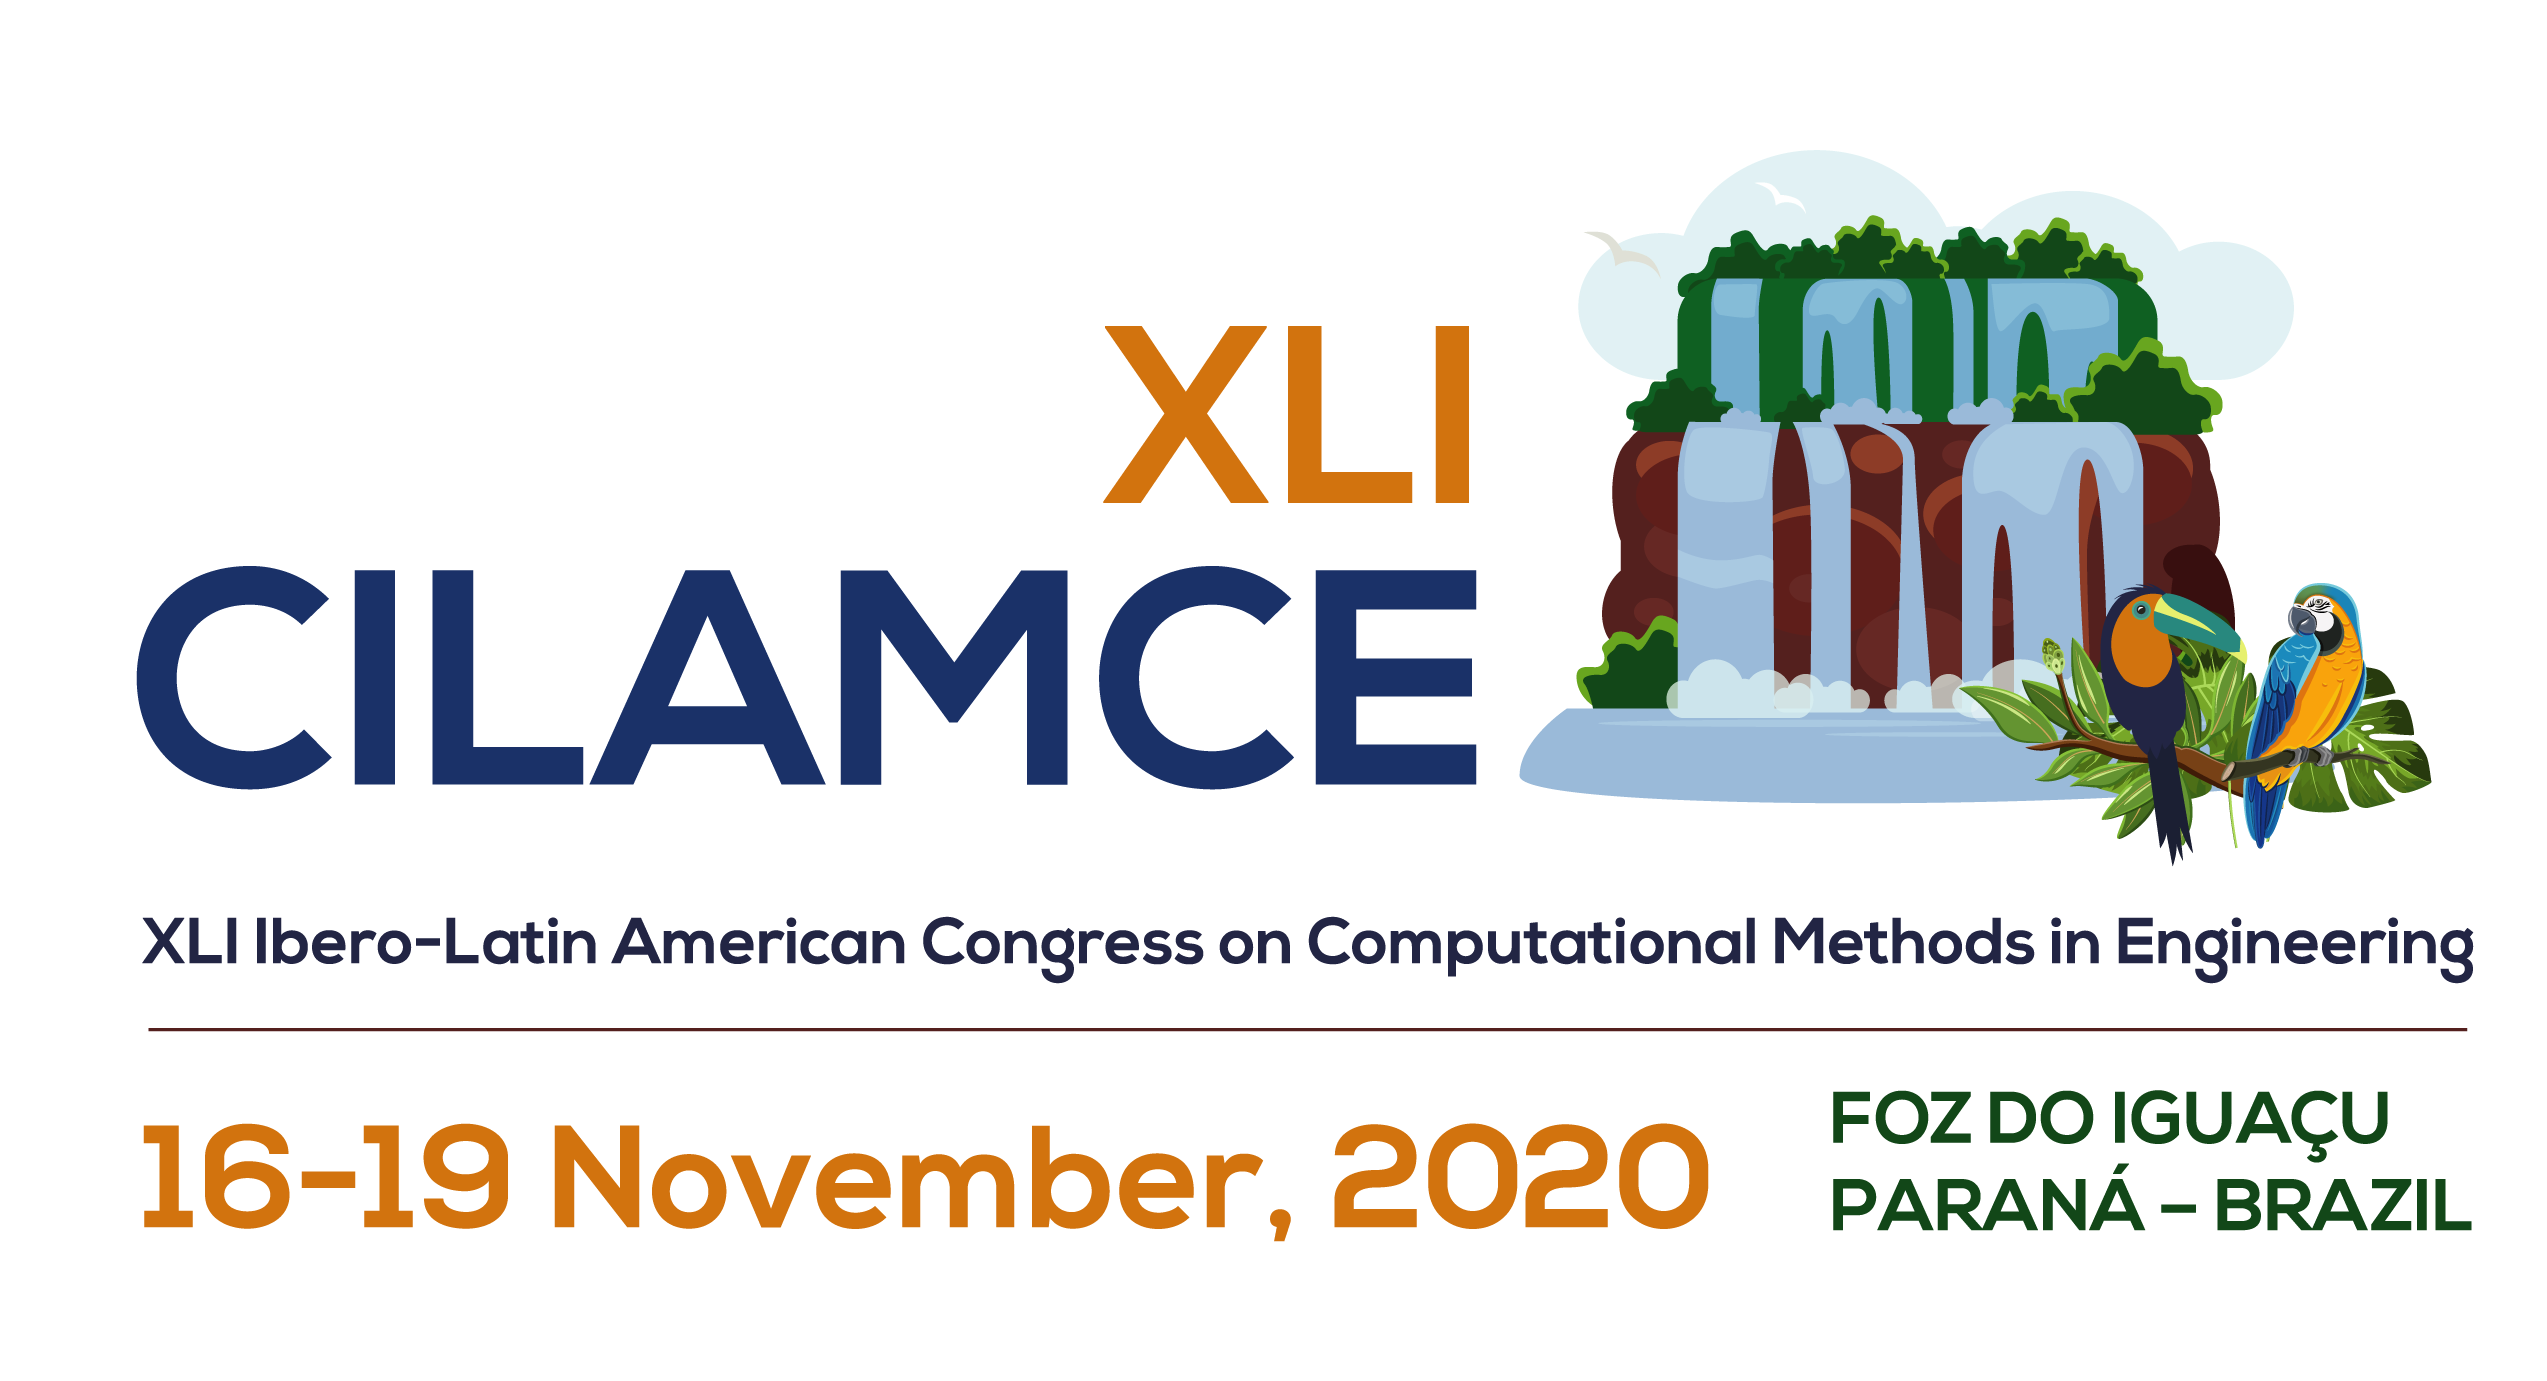
\includegraphics[width=5.5cm]{Figures/logoCILAMCE2020.png}
%scale=0.25
\end{figure}

% --------------------------------------------------------------------------
% TITLE OF PAPER
% --------------------------------------------------------------------------

\noindent
\textbf{\Large
Concrete compressive strength prediction with machine learning} 
\vspace{18pt} % <- keep this vertical space!

% --------------------------------------------------------------------------
% AUTHORS
% --------------------------------------------------------------------------

\noindent Pedro B. A. Moreira$^1$, Victor M. Silva$^1$

\vspace{18pt} % <- keep this vertical space!

\noindent $^1$\textit{Student, Dept. of Engineering, University Veiga de Almeida}

\noindent \textit{Avenida das Américas, 22631-004, Rio de Janeiro, Brazil}

\noindent \textit{pedrobermoreira@gmail.com}

\noindent $^2$\textit{Assistant Professor, Dept. of Engineering, IBMEC/RJ}

\noindent \textit{Avenida Armando Lombardi 940, 22640-000, Rio de Janeiro, Brazil}

\noindent \textit{victor.silva@professores.ibmec.edu.br}


\vspace{18pt} % <- keep this vertical space!

% --------------------------------------------------------------------------
% ABSTRACT
% --------------------------------------------------------------------------

\noindent \textbf{Abstract.}
TODO: REDUCE TO 200 WORDS, CURRENTRLY IT HAS 270. Compressive strength is the main characteristic of concrete. The correct prediction of this parameter means cost and time reduction. This work built predictive models for 6 different ages of concrete samples. A set of 1030 samples from previous studies was used, with 9 variables: compressive strength, age, and 7 ingredients. Another 6 variables were added to represent the proportions of the main ingredients in each sample (water/cement, fine aggregate/cement, coarse aggregate/cement, fine aggregate/coarse aggregate, water/coarse aggregate, and water/fine aggregate). The predictive models were developed in R language, using the caret package with the Parallel Random Forest algorithm and repeated cross-validation technique to optimize the parameters. The results were satisfactory and compatible with other studies using the same data set. The most important model, 28 days old, obtained a root mean square error (RMSE) of 4.717. The 3-day model obtained the best result, RMSE of 3.310. The worst result was the 56-day model, with RMSE of 5.939. The work showed that the compressive strength of concrete can be predicted. The choice of creating a model for each age, instead of using age as a predictor, allowed to get compatible results with the available data at each age. It was a promising alternative since good results were achieved by training with just one algorithm. This work facilitates exploration and new efforts to predict the compressive strength of concrete, it can be used as a baseline to predict with different algorithms or the combination of several.

\vspace{18pt} % <- keep this vertical space!

\noindent \textbf{Keywords:} Concrete, Compressive Strength, Machine Learning, Prediction

% --------------------------------------------------------------------------
\section{Introduction}\label{sec:introduction}
% --------------------------------------------------------------------------


Compressive strength is the main characteristic of concrete, measured by tests of international standards that consist of the breaking of specimens (\citet{Gambhir1990}). Measurement at 28 days is mandatory and represents the grade of the concrete. Knowing in advance what the result will be obtained for a given age, based on the proportions of its ingredients, is of great interest to concrete manufacturers, construction companies, and civil engineers.
 
The compressive strength is a nonlinear function of its ingredients and age, making it difficult to establish an analytical formula, although some formulas have already been proposed (\cite{Hasan2011}, \cite{Kabir2012}). However, most of the studies have build models including the age as a feature along with the ingredients, but because of the non linearity between the compressive strength and age, we have find the need of further investigation of models that separate the age and analyse only the ingredients, then specify for each age. 

Therefore, the present study aims at building predictive models for the concrete compressive strength at different ages using only it's ingredients as features.


% --------------------------------------------------------------------------
\section{Related work}\label{sec:introduction}
% --------------------------------------------------------------------------

TODO: Estou com dúvida, se coloco os resultados dos outros trabalhos aqui, porque são apresentados na seção de conclusão e discussão.

TODO: Essa seção ainda tem que ser mais desenvolvida.

TODO: Focar nos que foram publicados/peer review.

% \citet{Hasan2011} proposed a mathematical model to predict 28 day compressive strength from the results of tests of 7 and 14 days, and \citet{Kabir2012} from 7 days. These are analytical formulas, but use

The data set used in this study was the one used originally by \citet{Yeh1998}, and then by many othe works. \citet{Alshamiri2020} got good results with the regularized extreme learning machine (RELM) technique, and \citet{Hameed2020} got even better results with the Artificial Neural Networks and cross-validation technique. This set of samples is so well known that there are many pages on the internet of unpublished studies that use it and have good results, such as \citet{Abban2016}, \citet{Raj2018}, \citet{Modukuru2020} and \citet{Pierobon2018}. Later in this paper all studies are compared with the results found here.


% --------------------------------------------------------------------------
\section{Materials and methods}\label{sec:MaterialsAndMethods}
% --------------------------------------------------------------------------

% --------------------------------------------------------------------------
\subsection{Materials and reproducibility} \label{subsec:materialsandreproducibility}
% --------------------------------------------------------------------------

The methodology was carried out using RStudio software (\citet{RStudio}), an integrated virtual environment for code development in R language (\citet{RCore}). Throughout the process, all code executed was documented in the same order as its execution and pushed to the github repository (TODO: CREATE GITHUB REPO BIBLIO AND ADD HERE). The repository contains an extended version of this paper, including all the code, required packages and versions. In order to guarantee reproducibility, whenever there was code that uses probabilistic operations, a seed was defined before its execution, ensuring results consistency when running on another machine.

The main package used to build the machine learning models was the Caret Package (\citet{caret}). It provides all functionalities and utilities to build prediction models for any data set, has a straight and clear documentation that guides the process and provide around 200 different algorithms to build models. We used only one algorithm in this work, chosen by the highest probability to achieve the best possible result, according to \citet{Fernandez2014}, who compared 179 algorithms across 121 different databases, and find out that the most likely to achieve the best possible results is the Parallel Random Forest (called prRF in the caret).


% --------------------------------------------------------------------------
\subsection{TODO ...} \label{subsec:todo}
% --------------------------------------------------------------------------

...


% --------------------------------------------------------------------------
% \subsection{Obtaining the data} \label{subsec:Obtainingthedata}
% --------------------------------------------------------------------------

% --------------------------------------------------------------------------
% \subsection{Data preparation} \label{subsec:datapreparation}
% --------------------------------------------------------------------------

% --------------------------------------------------------------------------
% \subsection{Data visualization} \label{subsec:datavisualization}
% --------------------------------------------------------------------------

% --------------------------------------------------------------------------
% \subsection{Machine learning models} \label{subsec:machinelearningmodels}
% --------------------------------------------------------------------------

% --------------------------------------------------------------------------
\section{Results}\label{sec:Results}
% --------------------------------------------------------------------------
The test RMSE for each model in ascending order of age was 3.31, 4.36, 4.62, 4.72, 5.94 and 5.85 respectively. Table \ref{tab:results} presents the details and results of each model, including the naive one. Fig. \ref{fig:results} compares the actual and predicted values for the final models.

\vspace{8pt}
\begin{table}[!ht]
\centering
\caption{Final models}
\label{tab:results}
\vspace{6pt}
\begin{tabular}{ccccccc}
\hline
Model & mtry & CV & Repetitions & Naive RMSE (test) & Final RMSE (train) & Final RMSE (test)\\ \hline
3 days & 6 & 30 & 10 & 9.303229 & 3.905196 & 3.310370\\
7 days & 2 & 10 & 10 & 13.443646 & 4.475981 & 4.361987\\
14 days & 13 & 30 & 10 & 7.593319 & 5.136687 & 4.620515\\
28 days & 11 & 30 & 10 & 14.283824 & 5.847334 & 4.716698\\
56 days & 8 & 30 & 10 & 12.702112 & 6.702565 & 5.939163\\
100 days & 8 & 10 & 10 & 12.614652 & 6.381940 & 5.851088\\ \hline
\end{tabular}
\end{table}
\vspace{8pt}

\begin{figure}[!ht]
\begin{center}
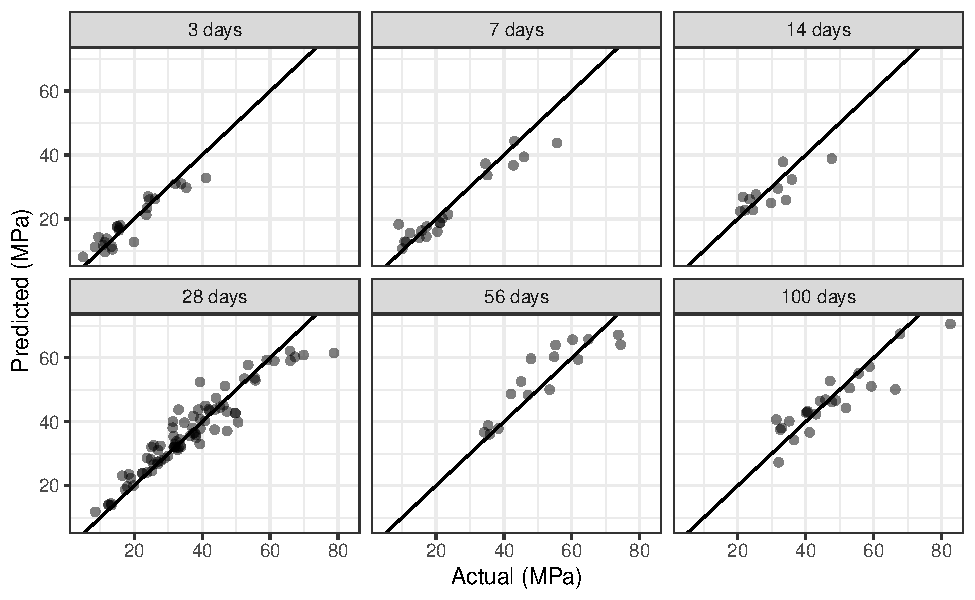
\includegraphics[scale=0.8]{Figures/results-comparison.pdf}
\vspace{12pt}
\caption{TODO:(O que tem que atualizar aqui?) Actual vs predicted values for each model}
\label{fig:results}
\end{center}
\end{figure}
\vspace{8pt}

% --------------------------------------------------------------------------
\section{Discussion and conclusion}\label{sec:DiscussionAndConclusion}
% --------------------------------------------------------------------------

The models built present satisfactory results and prove that the compressive strength of concrete can be predicted relatively easily.The alternative adopted, to create a model for each set of age proved to be a valid method, instead of using the age as a predictor along with the ingredients like the related studies with the same dataset. The adoption of this stratification achieved different results for each age group. However, the RMSE calculated in our work and the one obtained in the related works were close. Table \ref{tab:comparison} shows the comparison between these studies and the 28 days model developed here.

\vspace{8pt}
\begin{table}[!ht]
\centering
\caption{Comparison to other works with same dataset}
\label{tab:comparison}
\vspace{6pt}
\begin{tabular}{lclcc}
\hline
Author & Year & Algorithm & RMSE & Difference ({\%}) \\ \hline
\citet{Pierobon2018} & 2018 & 5 algorithms Ensemble & 4.150 & -12\\
\textbf{This work (28 day)} & \textbf{2020} & \textbf{Parallel Random Forest} & \textbf{4.717}  & \textbf{0}\\
\citet{Hameed2020} & 2020 & Artificial Neural Networks & 4.736 & 0\\
\citet{Raj2018} & 2018 & Gradient Boosting Regressor & 4.957  & +5\\
\citet{Modukuru2020} & 2020 & Random Forest Regressor & 5.080  & +8\\
\citet{Alshamiri2020} & 2020 & Regularized Extreme Learning Machine & 5.508 & +17\\
\citet{Abban2016} & 2016 & SVM with Radial Basis Function Kernel & 6.105 & +29\\ \hline
\end{tabular}
\end{table}
\vspace{8pt}


Following the line of reasoning of this work, the same hypothesis can be evaluated using other algorithms besides the one used here (Parallel Random Forest), as they can present better results. Another option is to create an ensemble of various algorithms, just like \citet{Pierobon2018}, but with the separation of age sets proposed here. In addition, this study can be reproduced with a larger dataset, ideally with a similar number of samples in each age group and a more homogeneous distribution of compressive strength.


%--------------------------------------------------------------------------
\vspace{20pt}
\noindent \textbf{Authorship statement.} The authors hereby confirm that they are the sole liable persons responsible for the authorship of this work, and that all material that has been herein included as part of the present paper is either the property (and authorship) of the authors, or has the permission of the owners to be included here. 

\vspace{20pt}
TODO: Na bibliografia, os ROI não entram por conta do modelo deles, que é inspirado no apa, o mais próximo que posso usar pra colocar o ROI é a chave "howpublished", mas ela não é usada em todas a bibliografias, depende do tipo, por exemplo @article, @inproceedings e @inbook não usam ela, acho que só a @misc usa (para publicacoes online), mas também não adianta porque as publicações online não tem ROI. Mas no geral atulizei as referencias e agora estão mais completas

\bibliography{bibliography}

\end{document}
% --------------------------------------------------------------------------